\section{Ejercicio 1 (BackTracking):}

En este ejercicio se nos pide resolver el problema utilizando un algoritmo de backtracking.

Backtracking es una técnica para buscar exhaustivamente todas las configuraciones del espacio de soluciones de un problema, para eso va generando las posibles soluciones constructivamente y va dejando atrás los candidatos cuando sabemos que no son válidos(que no pertenecen al espacio de soluciones válidas del problema).

Para este problema queremos buscar el minimo de numeros sin pintar para una secuencia de números de largo $n$. Ya que un número puede estar pintado de rojo, azul o sin pintar, y como tenemos $n$ números, podemos tener como máximo $3^n$ posibles combinaciones, aunque podrían ser menos ya que de esas combinaciones hay posibilidades que no son válidas como soluciones ya que puede ser que la subsecuencia de rojos no sea creciente o decreciente para la de azul. Una vez generadas todas estas soluciones, deberíamos encontrar la que menos numeros tiene sin pintar y esa va a ser la solución a nuestro problema(se nos pide la cantidad no qué combinación de rojos y azules).

Ya que estamos construyendo las distintas soluciones, empezamos decidiendo de qué color pintar el número primer número, rojo azul o sin pintar, para cada una de estas 3 decisiones vamos a pasar al siguiente número y repetir el proceso, así hasta llegar al final en el que vamos a tener como pintamos los numero y nos fijamos cuantos dejamos sin pintar. Una vez que tenemos todas las soluciones buscamos la óptima.

Se puede implementar este algoritmo de manera recursiva, dado el arreglo de números, el índice, y cuál fue el último rojo y último azul pintado(si hay), devuelve la mínima cantidad de números sin pintar dentro de las posibilidades. Pedimos el último rojo y el último azul porque no me importa saber cómo los pinte si no los últimos ya que eso me va a dar la limitante de si el próximo número lo puedo pintar de rojo o azul(y descartamos los que no pude pintar). Entonces esta función recursiva guarda los resultados del índice siguiente para las 3 posibilidades(rojo, azul y sin pintar), se fija cual es la menor y devuelve esa(si es la que no se pinta tiene que sumarle uno), excepto que sea el caso basó en el que no hay indice siguiente y devolvemos 0 si podemos pintarlo(0 elementos sin pintar en un arreglo que contiene sólo al último elemento pintado de cualquier color) o 1 si no lo pudimos pintar, y despues se van a ir llenando las anteriores llamadas con estos casos bases.

\subsection*{Pseudocodigo}
\begin{algorithm}[H]
\NoCaptionOfAlgo
	\KwData{	
	arreglo = el arreglo de numeros entero\\
	n = el tamaño del arreglo
	\KwResult{La cantidad minima de numeros sin pintar para una secuencia de numeros de largo n}
	\caption{\algoritmo{ej}{int arreglo[], n}{int}}
		\tcc{Empezamos el backtracking desde el primer indice(0) y no inicializamos todavia el ultimo rojo y el ultimo azul}
		res $\leftarrow$ BT(0, arreglo, n, NULL, NULL)\\
	}
\end{algorithm}
\begin{algorithm}[H]
\NoCaptionOfAlgo
	\KwData{
	i = indice actual a pintar\\
	arreglo = el arreglo de numeros entero\\
	n = el tamaño del arreglo\\
	ultimoRojo = el ultimo numero que se pinto de rojo(NULL si no se pinto ninguno)}
	\KwResult{La cantidad minima de numeros sin pintar a partir de i hasta n}
	\caption{\algoritmo{BT}{int i, arreglo[], n, ultimoRojo, ultimoAzul}{int}}

	numeroActual $\leftarrow$ arreglo[i]\\
	\eIf{ i = $n-1$ }{
		\tcc{Si el indice es el ultimo numero entonces estamos en el caso base}
		\tcc{Tenemos que fijarnos si podemos pintarlo}
		\eIf { ultimoRojo = NULL \textbf{or} ultimoAzul = NULL \textbf{or} ultimoRojo $<$ numeroActual \textbf{or} ultimoAzul $>$ numeroActual }{
			res  $\leftarrow$ 0
		}{
			\tcc{No lo podemos pintar porque no seria una solucion valida entonces devolvemos 1}
			res  $\leftarrow$ 1
		}
	}{	
		int minSiRojo, minSiAzul, minSinPintar\\
		\If{ ultimoRojo = NULL \textbf{or} ultimoRojo $<$ numeroActual} {
			\tcc{Si lo podemos pintar el numero actual de rojo osea si es mas grande que el anterior rojo pintado, o si es el primero rojo en pintarse, y cambiamos el ultimoRojo por este numero}
			minSiRojo $\leftarrow$ BT(i+1, arreglo, n, numeroActual, ultimoAzul)
		}
		\If{ ultimoAzul = NULL \textbf{or} numeroActual $<$ ultimoAzul} {
			\tcc{Lo mismo con el azul}
			minSiAzul $\leftarrow$ BT(i+1, arreglo, n, ultimoRojo, numeroActual)
		}
		\tcc{Calculamos tambien si no lo pintamos y al resultado le sumamos uno porque este no lo pintamos}
		minSinPintar $\leftarrow$ BT(i+1, arreglo, n, ultimoRojo, ultimoAzul) + 1\\
		\tcc{retornamos el minimo de ambos(considerando que la func min es O(1) y si es nulo la variable no lo considera)}
		res $\leftarrow$ min(minSiRojo, minSiAzul, minSinPintar)
	}

\end{algorithm}

\subsection*{Análisis de Complejidad}
Ya dijimos que la cantidad de combinaciones posibles son $3^n$, y podemos decir que este algoritmo recorre como máximo todas ellas porque empieza desde el índice 0 y por cada número del arreglo prueba las 3 combinaciones(nada más las válidas), entrando recursivamente al índice siguiente(i+1) y esos lo van a repetir hasta llegar al caso base que sería llegar al último índice. Ahora, cada llamada recursiva hace una cantidad de operaciones O(1) constantes (sumar, comparar, mínimo) y si no es el caso base además hace 3 llamadas recursivas en peor caso, pero reduciendo el n. Esto nos hace quedar que la complejidad de la función recursiva es $T(n) = 3T(n-1) + O(1)$ con $T(0) = 1$ como el caso base, que se puede demostrar fácilmente (por inducción) que es $O(3^n)$ para el peor caso. Otra forma de llegar es ver el árbol de ejecución de la recursión, cada nodo desprende tres nodos hijos, vamos a tener un árbol de altura n, y como es un árbol ternario tenemos $3^n$ hojas, que son nuestras soluciones. Esta complejidad se considera exponencial y es muy mala para instancias grandes.
Obviamente esto no pasa siempre, porque no siempre es posible entrar calcular las 3 posibilidades, de hecho es muy probable que no se pueda, supongamos que ya pintamos un numero de rojo y un número azul, para que entre a las tres bifurcaciones el número este tiene que ser mayor al rojo y menor al azul, osea que el azul tiene que ser mayor que el rojo y ademas el numero actual tiene que estar en el medio, ahora cuando sigamos con el próximo número esta brecha se va a haber achicado entonces va a ser menos probable que el número caiga en el medio de ambos.

\subsection*{Experimentación Computacional}
\subsubsection*{Instancias Aleatorias}
Se corrió una experimentación, sobre el código realizado en c++, generando arreglos aleatorios de tamaño n, y los números tienen una distribución uniforme donde el mínimo es 0 y el máximo es 2 veces n, esto se hizo así, para que exista una buena probabilidad de que haya números repetidos, ya que si por ejemplo hay un número repetido 3 veces no existe posibilidad de que el óptimo sea 0, así agregando casos malos a la experimentación. Se probaron arreglos de tamaño: 1, 2, 5, 10, 15, 20, 25, 30, 35 y 40. De cada uno de estos tamaños se computaron 30 arreglos diferentes, de estos 30 se tomo el promedio.

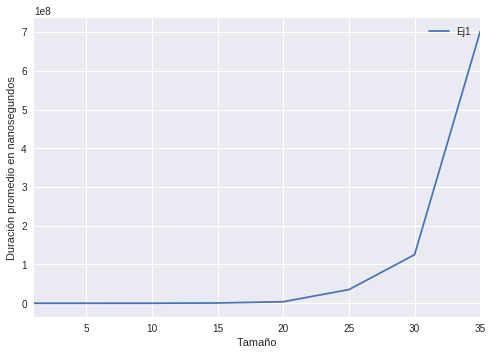
\includegraphics[scale=0.5]{ej1Random1-40.png}\\
Como podemos ver en el gráfico lo que tarda en resolver el problema aumenta exponencialmente a medida que crece el tamaño del arreglo, de hecho en promedio para calcular el arreglo de tamaño 40 es TODO segundos que es mucho, y para el de 35 tardó 0,701732075 segundos casi TODO veces más. Para seguir haciendo énfasis en que cada vez tarda más hagamos zoom para los primeros dato\\ 
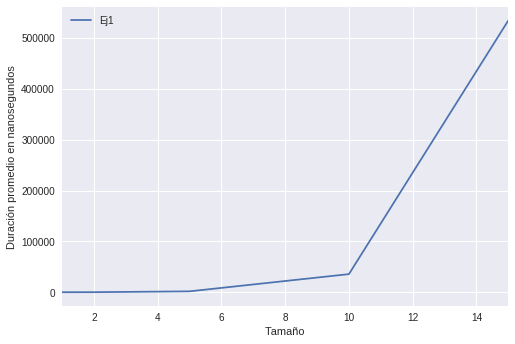
\includegraphics[scale=0.5]{ej1Random1-5.png}\\
En este gráfico también podemos apreciar como va creciendo exponencialmente(en el otro grafico parecia que al principio era constante la duración). En este caso tenemos que en promedio para los arreglos de tamaño 5 tardan 0,001741 milisegundos y para los de tamaño 10 tarda 0,035622 milisegundos casi 20 veces más.\\

Conclusión si bien es viable para instancias chicas, es muy ineficiente y tarda mucho cuando las instancias empiezan a ser más grande

